\documentclass{article}
\usepackage[letterpaper]{geometry}
\geometry{verbose,tmargin=1in,bmargin=1in,lmargin=1in,rmargin=1in}

\usepackage[utf8]{inputenc}
\usepackage{amsmath}
\usepackage{float}
\usepackage{listings}
\usepackage{graphicx}
\usepackage{enumitem}

\title{CIS 419/519: Homework 3}
\author{\{Yupeng Li\}}
\date{02.20.2020}

\begin{document}
    \maketitle
    Although the solutions are entirely my own, I consulted with the following people and sources while working on this homework:
    
    \section{Logistic Regression}
    	\subsection{Implementation}
	This section is done in the python file with both L1 regularization and L2 regularization implementations.
	
	\subsection{Testing Your Implementation}
	In this section, the implementation of the logistic regression is tested dataframe and yields a similar result in the assignment PDF. The results are in the figure below:
		\begin{figure}[H]
			\caption{Graph under L2 norm and $\lambda$ = 1E-9}
			\centering
			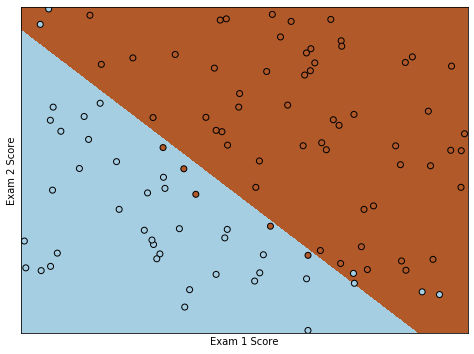
\includegraphics[width=8cm]{LinearL2norm.png}
		\end{figure}

	\subsection{Analysis}
	In this part, we would compare the results for logistic regression based on different $\lambda$ and under situations of 1 norm and 2 norm:
		\begin{figure}[H]
			\caption{Graph under L2 norm and $\lambda$ = 10}
			\centering
			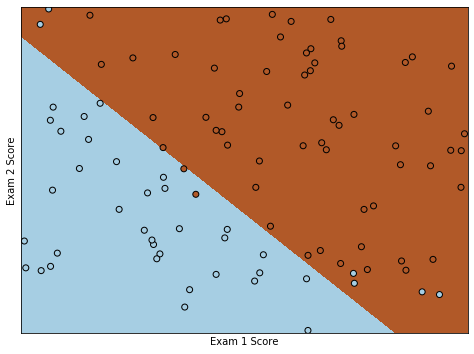
\includegraphics[width=8cm]{LinearL2norm10.png}
		\end{figure}
		\begin{figure}[H]
			\caption{Graph under L1 norm and $\lambda$ = 1E-9}
			\centering
			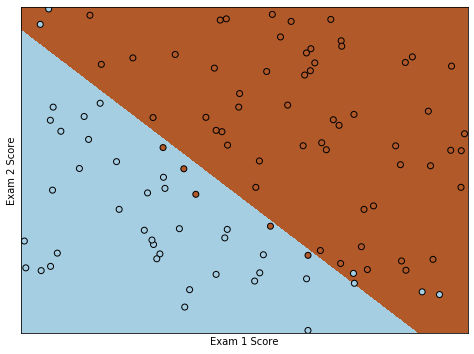
\includegraphics[width=8cm]{LinearL1norm0.png}
		\end{figure}
			\begin{figure}[H]
			\caption{Graph under L2 norm and $\lambda$ = 10}
			\centering
			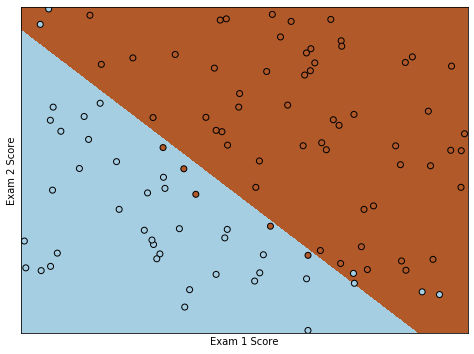
\includegraphics[width=8cm]{LinearL1norm10.png}
		\end{figure}
		\\
		
	We can see from the figures that, with almost 0 regularization constant, both L1 norm result and L2 result are exhibiting similar pattern with no significant difference. While when the regularization constant is raised to 10, the L2 regularization pushes the decision boundary slightly forward towards negative while the results of L1 regularization stays almost the same.
	
	\subsection{Learning a non-linear decision surface}
	This part is in the submitted .py file
	The following graph demonstrates how the non-linear decision surface works with almost 0 L2 regularization
	\begin{figure}[H]
			\caption{Graph under L2 norm and $\lambda$ = 1E-9}
			\centering
			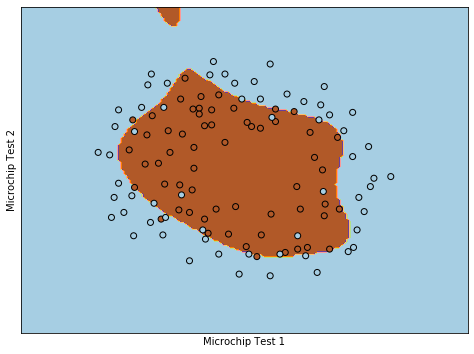
\includegraphics[width=8cm]{NonlinearL2norm0.png}
		\end{figure}
	\section{Comparing Algorithms}
		\subsection{Logistic Regression Adagrad}
	
	




        
\end{document}